\chapter{Introduction}\label{chapter:introduction}
The level-I assessment will assume key variables such as propeller efficiency to be constant. The level-II assessment will use empirical estimations for key variables. Lastly, the level-III assessment will use some mid-fidelity models such as BEM to assess propeller performance. The code for this project can be accessed on GitHub\footnote{\url{https://github.com/jexalto/ElysianMonorepo}}.

The purpose of this document is to give a comprehensive overview of three different take-off performance estimation methods. These methods are consequently built into a computer program, that can evaluate take-off distance characteristics for a certain set of inputs. Such a model is relevant because often aircraft design is led by landing and take-off conditions and performance. Therefore, properly modeling the LTO cycle will give further insights in the requirements for other subsystems. The goal of this report is to produce a graph like \autoref{fig:schematic_takeoff}, which could be found in Torenbeek. Through such a graph the balanced field length can be obtained. Furthermore, it is important to validate the model since important design choices will depend on this work.

\begin{figure}[!ht]
    \centering
    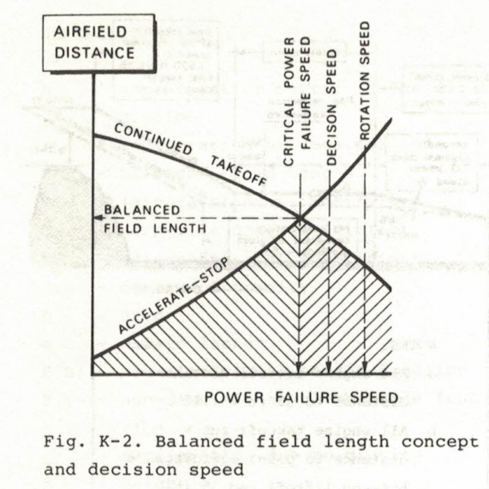
\includegraphics[width=0.5\linewidth]{figures/s_distance.png}
    \caption{Schematic of the take-off phase and velocity nomenclature}
    \label{fig:schematic_takeoff}
\end{figure}